Consider a cluster of computers that is serving a stream of tasks which are
distributed across the cluster by a resource manager. Each task consumes certain
resources during its execution; examples include the \up{CPU} and memory usage
over time. The cluster has an adequate monitoring facility deployed so that the
resource usage of the tasks is at one's disposal.

The resource-usage trace of task $i$ is defined as a sequence of equally spaced
$d$-dimensional measurements in time, which we shall represent as the following
tensor of size $l_i \times d$:
\begin{equation} \elab{trace}
  x_i = \left(x_{i0}, \dots, x_{ik}, \dots, x_{i,l_i - 1}\right)
\end{equation}
where $x_{ik}$ is the measurement taken at time $t_{ik}$, and $l_i$ denotes the
length of the sequence. Such a sequence is called fine-grained data as it
contains multiple measurements over the execution of the task as opposed to
having only one aggregative measurement such as the average or maximum value.

Suppose further that the current time is $t_{ik}$. This means that $x_{i0},
\dots, x_{ik}$ of task $i$ are known. Given these previous values of the trace,
our goal is to estimate its next $h$ values, which we shall denote by
$\hat{x}_{i,k + 1}, \dots, \hat{x}_{i,k + h}$. Such an estimation is called a
long-range prediction as it provides multiple future values as opposed to only
one. This operation is to be performed for each active task of interest at any
time moment of interest.

In order to attain the objective, we reside to learning from historical data.
Specifically, it is first assumed that there is a data set of resource-usage
traces available, and that these past resource-usage traces are representative
of the future ones:
\begin{equation} \elab{traces}
  X = \{ x_i: i = 0, \dots, n - 1 \}
\end{equation}
where $n$ is the total number of traces, and $x_i$ is as in \eref{trace}. We
apply machine learning to the data in order to construct an adequate model
offline, and this model is then used in order to make predictions at runtime. We
specifically aim at investigating the utility of the state-of-the-art in machine
learning; to this end, we use recurrent neural networks \cite{goodfellow2016}.

\begin{figure*}
  \centering
  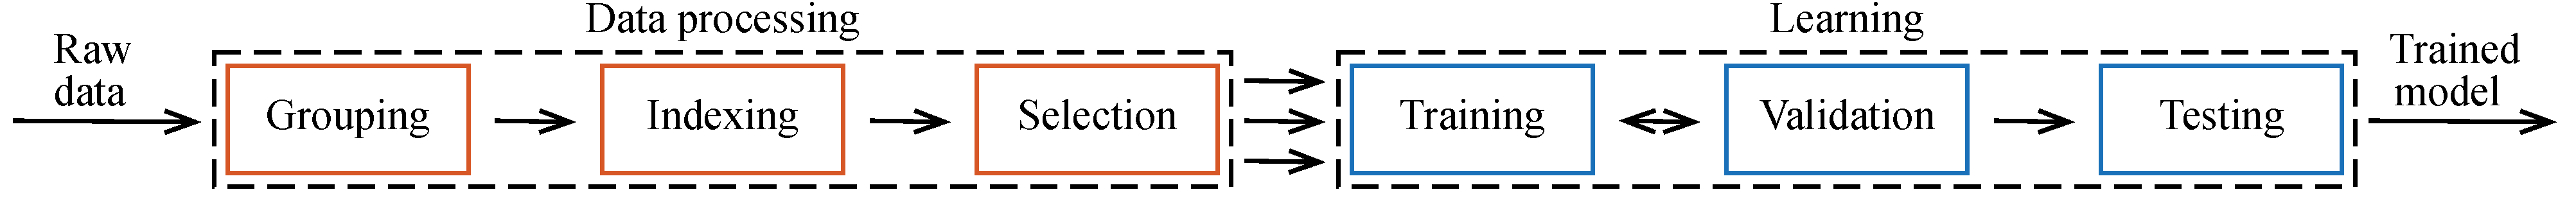
\includegraphics[width=1.0\textwidth]{include/assets/figures/overview.pdf}
  \vspace{-2.0em}
  \caption{
    Overview of our workflow. The data-processing and learning stages are
    described in \sref{data} and \sref{learning}, respectively.
  }
  \vspace{-1.5em}
  \flab{overview}
\end{figure*}

Lastly, in order for learning to be possible, the fine-grained resource-usage
traces that we consider have to have a certain structure (not purely random),
which could be extracted and used for intelligent prediction. An important
question is whether real-life traces of this kind, at all, exhibit such a
structure. Investigating this question is part of our objective in this work.
